% Copyright page
\thispagestyle{empty}
% \null\vfill

\begin{center}
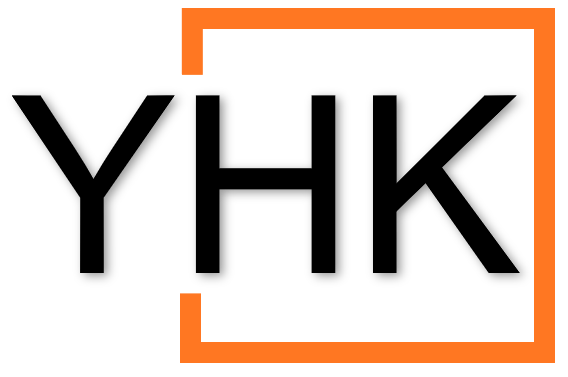
\includegraphics[width=0.2\linewidth,keepaspectratio]{YHK_Color_OutOfTheBox_tight} \\[1.5em]

\textbf{\Huge सहज जीवन}\\ [0.5em]
{\small(मराठीतील कदाचित पहिले मुक्त-स्रोत, सार्वजनिक, सहकारी आणि अद्ययावत  पुस्तक)}\\[0.5em]

अनुवादक-लेखक: \textbf{{\large \ldots आणि  डॉ. योगेश हरिभाऊ कुलकर्णी}}\\[1.5em]
\end{center}

\vspace{1.5em}

\begin{flushleft}

प्रकाशक: डॉ. योगेश हरिभाऊ कुलकर्णी (self-published at Notion Press)\\
पत्ता:  पाषाण ,  पुणे ८ \\
फोन:  +91 9890251406\\
ईमेल: yogeshkulkarni@yahoo.com\\[1.5em]

\vspace{0.5em}

प्रथम आवृत्ती: २०२५\\[0.5em]

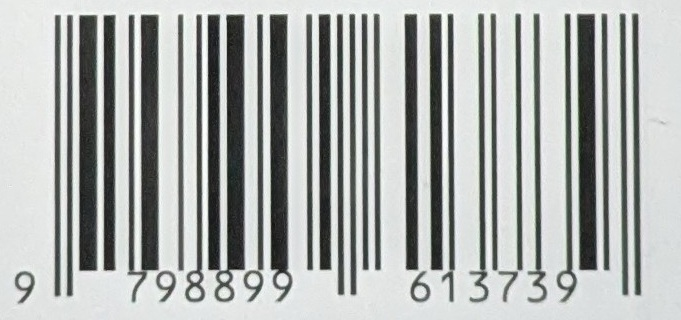
\includegraphics[width=0.3\linewidth,keepaspectratio]{sahajjeevan_isbn} \\ [0.5em]
ISBN-13 ‏ : ‎ XXX-XXXXXXX\\[1.5em]

कॉपीराइट-मुक्त © २०२५ डॉ. योगेश हरिभाऊ कुलकर्णी\\[0.5em]

{\textit{सर्व हक्क सार्वजनिक. या पुस्तकाचा कोणताही भाग प्रकाशकाच्या लेखी परवानगीशिवाय कोणत्याही स्वरूपात पुनर्मुद्रित किंवा पुनर्प्रकाशित करता येईल.}}\\[1.5em]

{\large Legal Notice:}\\
{\textit{This entire work is uncopyrighted. No rights reserved. Any part of this publication may be reproduced, distributed, or transmitted in any form or by any means, including photocopying, recording, or other electronic or mechanical methods, without the prior written permission of the publisher.}}
\end{flushleft}
\vfill\null
\clearpage

\begin{dedication}
मुक्त-स्रोत (`ओपन-सोर्स') चळवळीस  समर्पित  
\end{dedication}

\clearpage

\chapter*{पुस्तकाविषयी}
हे पुस्तक प्रामुख्याने दोन भागात आहे.  पहिल्या भागात लीओ बाबाउटा यांच्या 'द एफर्टलेस लाईफ' या पुस्तकाचा स्वैर अनुवाद आहे.  मूळ पुस्तक जगभरातील वाचकांच्या मदतीने इंग्रजीत सार्वजनिक पद्धतीने लिहिले गेले होते.  मूळ पुस्तकप्रमाणेच  हे भाषांतरसुद्धा  कोणत्याही हक्काधिकाराशिवाय (Uncopyrighted) उपलब्ध ठेवले आहे.  तर दुसऱ्या भागात लेखकासकट इतर सहयोग्यांनी पाठवलेले विचार असणार आहेत.  हा दुसरा भाग अद्ययावत (live) असणार आहे .  याचा प्रपंचाचा उद्देश मराठी वाचकांना ``सहज जीवन'' जगण्यासाठी मार्गदर्शन मिळावे हा आहे. 
